% !TeX root=../../../main.tex
\chapter{پیاده‌سازی}
%\thispagestyle{empty} 
برای بررسی و امکان‌سنجی پیاده‌سازی روش ارائه شده در این پژوهش
یک نمونه‌ی اولیه%
\lf{Prototype}
از ابزار
EStResT \lf{
    \href{https://github.com/seyhani/causality/tree/dev/estrest}
    {https://github.com/seyhani/causality/tree/dev/estrest}
}
پیاده‌سازی شده است.

این ابزار با استفاده از زبان پایتون نسخه ۸.۳ پیاده‌سازی شده است.
در این پیاده‌سازی امکان توصیف یک ساختمان‌ رویداد و سپس بررسی اینکه
چه مقداری از متغیر‌ها می‌توانند به عنوان علت خطا در نظر گرفته شوند وجود دارد.
در این ابزار توصیف رفتار‌های نا امن در یک ساختمان رویداد مطابق تابع
\ref{eq:unsafe}
در نظر گرفته می‌شود.

چگونگی استفاده از این ابزار را با ذکر یک مثال بررسی می‌کنیم.
برای سادگی فرض کنید 
$a,b,c,d$
عملیات‌های زبان نت‌کت پویا باشند.
$\mr{E}$
را ساختمان رویداد معادل برنامه‌ی نت‌کت پویای 
$a;b \oplus c;d$
در نظر می‌گیریم.
پیکربندی‌های این ساختمان رویداد در شکل 
\ref{ex:impl:es}
مشخص شده است.
فرض کنید در این ساختمان رویداد به دنبال پیدا کردن علت
وجود پیکر بندی
$\s{(0,0,a),(0,1,0,b)}$
در ساختمان رویداد باشیم.
بنابراین می‌توانیم
$C = \left\{  \s{(0,0,a),(0,1,0,b)}\right\}$
را به عنوان مجموعه‌ی پیکر‌بندی‌های نا امن در نظر 
بگیریم و مطابق تابع
\ref{eq:unsafe}
رفتار‌های نا امن را توصیف کنیم.
\begin{figure}
    \centering
    \begin{tikzpicture}
        \crd[above]{0}{0}{$\emptyset$}
        \crd[left]{-2}{1}{$\s{(0,0,a)}$}
        \crd[left]{-2}{2}{$\s{(0,0,a),(0,1,0,b)}$}
        \crd[right]{2}{1}{$\s{(1,0,c)}$}
        \crd[right]{2}{2}{$\s{(1,0,c),(1,1,0,d)}$}
        \draw [ultra thick] (0,0) -- (-2,1);
        \draw [ultra thick] (-2,1) -- (-2,2);
        \draw [ultra thick] (0,0) -- (2,1);
        \draw [ultra thick] (2,1) -- (2,2);
    \end{tikzpicture}
    \caption{نمودار پیکربندی‌های 
    $\mr{E}$
    }
    \label{ex:impl:es}
\end{figure}
\begin{figure}
    \centering
    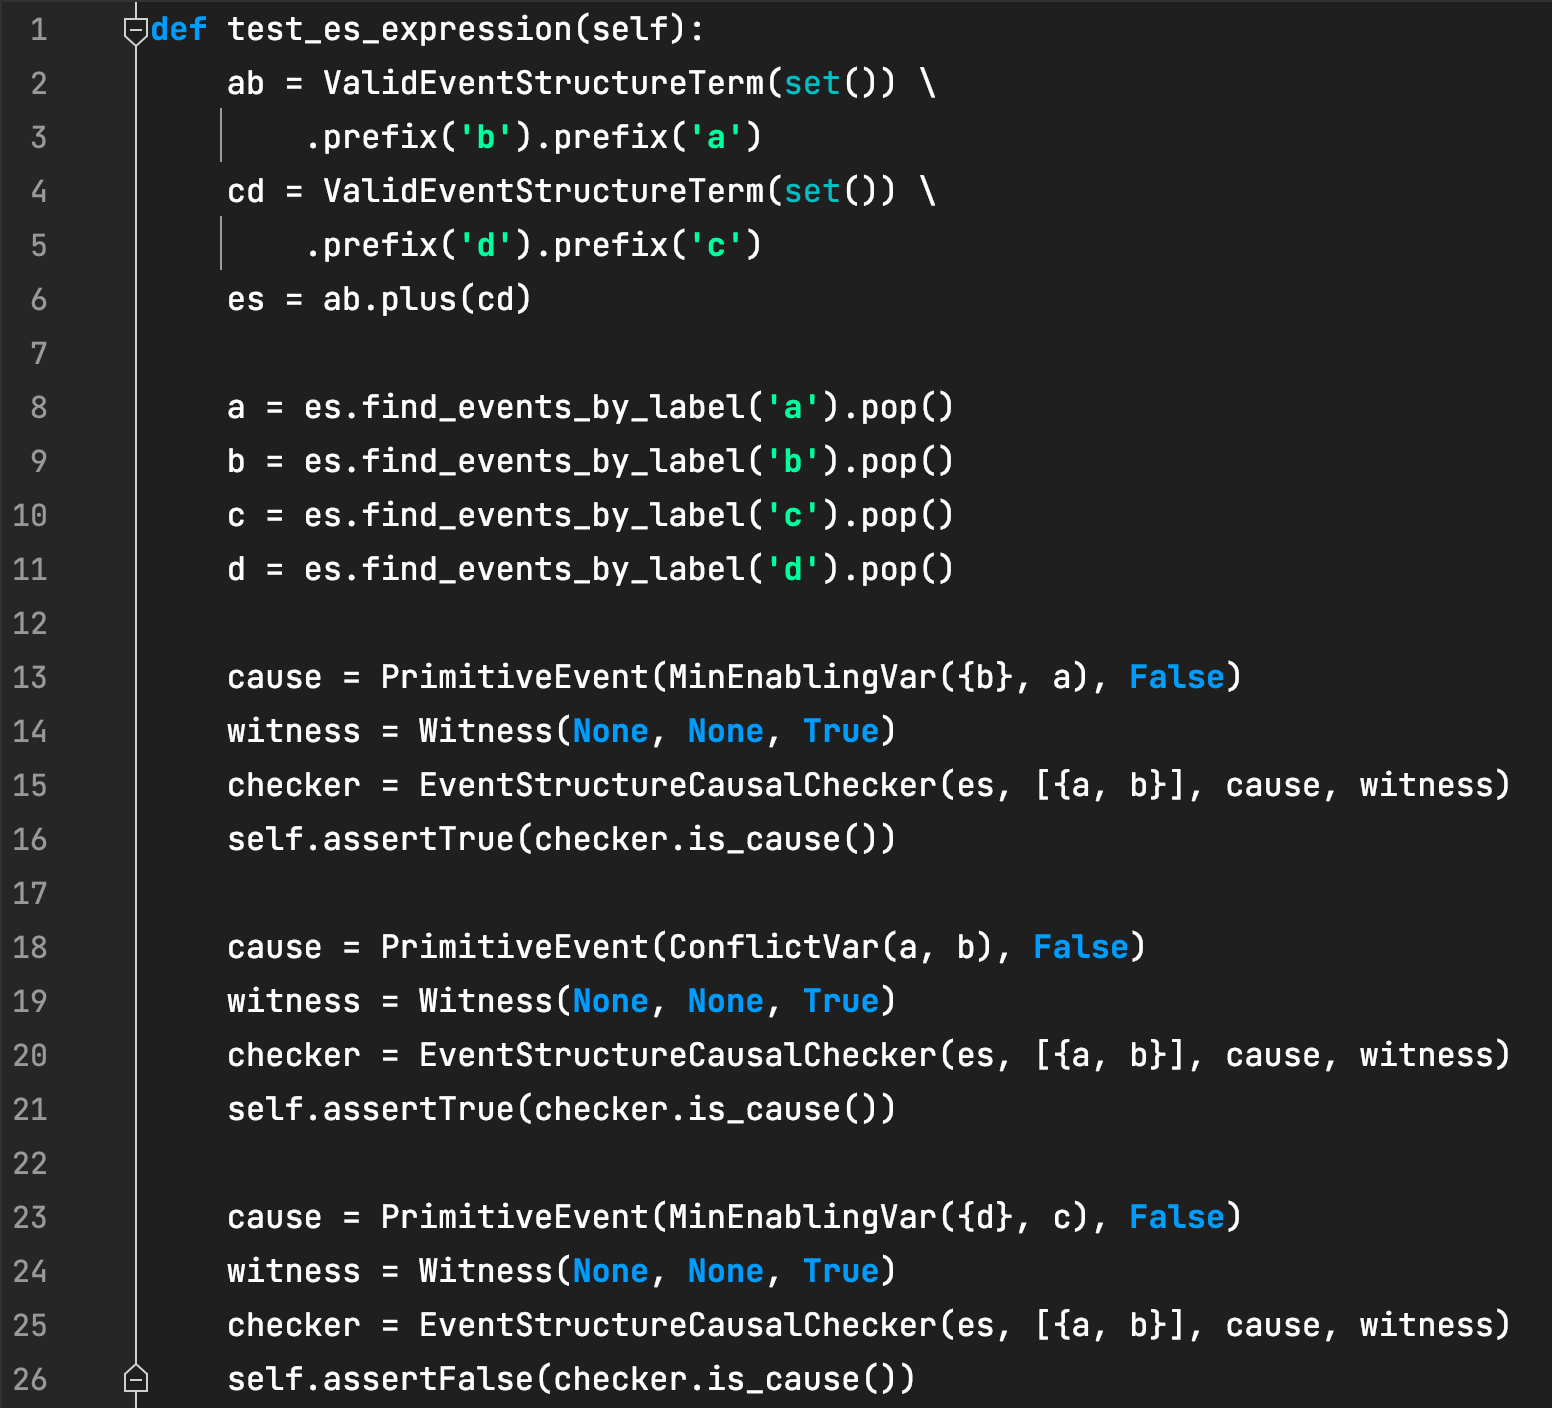
\includegraphics[width=15cm]{impl.png}
    \caption{بررسی علت‌ها در 
        EStResT 
    }
    \label{ex:impl:code}
\end{figure}
در قطعه کد 
\ref{ex:impl:code}
چگونگی استفاده از ابزار 
EStResT
برای بررسی علت‌های این مثال مشخص شده است.

در خطوط ۲ تا ۶ ساختمان رویداد معادل با 
$\mr{E}$
ساخته شده است.
در خطوط ۸ تا ۱۱ برای خوانایی بیشتر کد، رویداد‌های متناظر با هر یک از برچسب‌های 
$a,b,c,d$
در ساختمان رویداد پیدا شده‌اند و به متغیر‌های مناسب اختصاص داده شده‌اند.
خطوط ۱۳ تا ۱۶ چگونگی بررسی یک علت را مشخص می‌کنند.
ابتدا در خط ۱۳،
$M_{\s{b},a} = \F$
به عنوان علت تعریف شده است.
سپس شاهدی به شکل 
$(\e,\e,\T)$
در نظر گرفته شده است.
در نهایت در خطوط ۱۵ و ۱۶ بررسی شده است که آیا 
$M_{\s{b},a} = \F$
علت وجود
$\s{(0,0,a),(0,1,0,b)}$
در پیکربندی‌های ساختمان رویداد است یا خیر.
در اینجا 
EStResT
شرط‌های علت واقعی را مطابق تعریف 
\ref{def:extended}
بررسی می‌کند و
به درستی 
$M_{\s{b},a} = \F$
به عنوان یک علت واقعی در نظر می‌گیرد.
در ادامه‌ی این قطعه کد 
$C_{a,b} = \F$
و 
$M_{\s{d},c} = \F$
به عنوان علت مورد بررسی قرار گرفته‌اند.
این قطعه کد به عنوان یک متد تست با استفاده از کتابخانه‌ی 
unittest
در مجموعه‌ی تست‌های ابزار 
EStResT
پیاده‌سازی شده است.

\section{کبمودها و کار‌های پیش‌رو}
در این بخش چند مورد از کمبود‌های این ابزار و گام‌های پیش‌رو برای 
توسعه آن را مورد بحث قرار می‌دهیم.

\subsection{ترجمه عبارت‌های 
نت‌کت پویا
}
در این نمونه‌ی اولیه امکان ترجمه‌ی یک رشته
\lf{String}
از عبارت‌های نت‌کت پویا وجود ندارد.
این مساله سبب می‌شود که همانند قطعه کد
\ref{ex:impl:code}،
برای توصیف یک عبارت نت‌کت پویا نیاز به نوشتن کد و فراخوانی متد باشد.
به همین دلیل افزودن امکان ترجمه‌ی مستقیم یک رشته شامل عبارت‌های نت‌کت پویا به 
ساختمان رویداد برای تسهیل استفاده آن برای کاربر یکی از گام‌های بعدی برای توسعه این ابزار است.

\subsection{بهینه‌سازی}
در این نمونه‌ی اولیه از ابزار 
EStResT
سعی شد تا پیاده‌سازی تا جای ممکن ساده و به دور از پیچیدگی باشد تا امکان توسعه و تغییر آن در صورت لزوم وجود داشته باشد.
اما این مساله موجب می‌شود تا این پیاده‌سازی بهینه نباشد و استفاده
از این ابزار، حتی برای ساختمان رویداد‌های ساده‌ای مانند مثال‌های 
بخش
\ref{section:examples}
،
کاربردی نباشد.
به همین دلیل در گام بعدی توسعه‌ی این ابزار لازم است که تا جای ممکن 
الگوریتم‌های بررسی علت و تولید ساختمان رویداد مورد
 بهینه‌سازی قرار گیرند.